
\newproblem{10d}
{
	Solve by graphing the given system of equations. Be sure to label axes with $x$, $y$, and with numbers. Identify and label the intersection point. $$\begin{cases}3x-y=5\\ 2x-3y=-6\end{cases}$$ \begin{onlyproblem}\begin{center}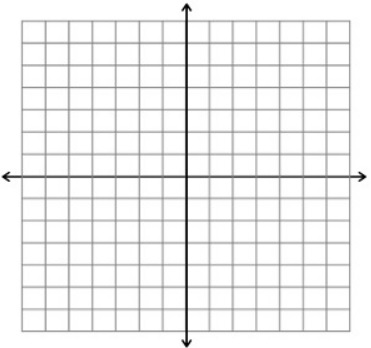
\includegraphics{fig-graphpaper.png}\end{center}\end{onlyproblem} \begin{onlysolution}\begin{center}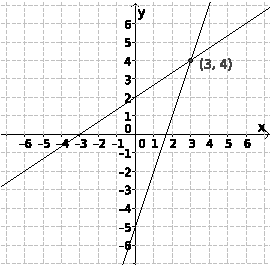
\includegraphics{fig095-10-d-answer}\end{center}\end{onlysolution}
	
}
{
	\begin{tabular}{l r}
	Correct system is graphed & award 2 pts\\
	Axes are labeled & award 1 pt\\
	Intersection point $(3,4)$ & award 2 pts
	\end{tabular}
}
